\begin{figure}[htpb]
    \centering
    \begin{tikzpicture}
        \begin{axis}[axis on top,smooth,
                axis line style=very thick,
                axis x line=bottom,
                axis y line=left,
                ymin=-5,ymax=5,xmin=-5,xmax=5,
                xlabel=$x_1$, ylabel=$x_2$,grid=major
            ]
            % \addplot[name path global=firstline,very thick, domain=-10:10]{3-x};
            % \addplot[name path global=secondline,very thick, domain=-10:10]{-5+2*x};
            % \addplot[name path global=thirdline,very thick, domain=-10:10]{3/2+x/2};
            \addplot[name path global=firstline, very thick, domain=-1:5]{2-x};
            \addplot[name path global=secondline, very thick, domain=-1:5]{-1};
            \addplot[name path global=thirdline, very thick, domain=-1:5]{-1-x};
            \fill[name intersections={of=firstline and secondline,by=point1},
                name intersections={of=firstline and thirdline,by=point2},
                name intersections={of=secondline and thirdline,by=point3},
            ][very thick,draw=orange,pattern=crosshatch dots,pattern color=green!60!white](point1)--(point2)--(point3)--(point1);
        \end{axis}
    \end{tikzpicture}
    \label{fig:p3:c1}
\end{figure}

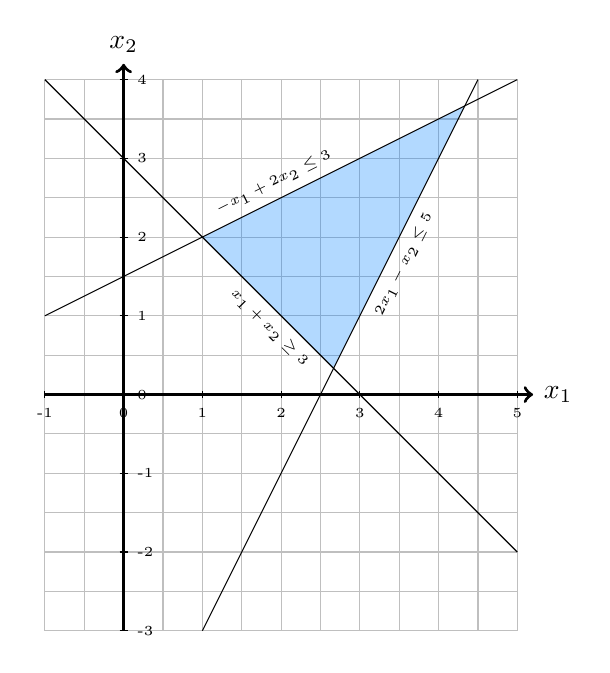
\begin{tikzpicture}

    \draw[gray!50, thin, step=0.5] (-1,-3) grid (5,4);
    \draw[very thick,->] (-1,0) -- (5.2,0) node[right] {$x_1$};
    \draw[very thick,->] (0,-3) -- (0,4.2) node[above] {$x_2$};

    \foreach \x in {-1,...,5} \draw (\x,0.05) -- (\x,-0.05) node[below] {\tiny\x};
    \foreach \y in {-3,...,4} \draw (-0.05,\y) -- (0.05,\y) node[right] {\tiny\y};

    \fill[blue!50!cyan,opacity=0.3] (8/3,1/3) -- (1,2) -- (13/3,11/3) -- cycle;

    \draw (-1,4) -- node[below,sloped] {\tiny$x_1+x_2\geq3$} (5,-2);
    \draw (1,-3) -- (3,1) -- node[below left,sloped] {\tiny$2x_1-x_2\leq5$} (4.5,4);
    \draw (-1,1) -- node[above,sloped] {\tiny$-x_1+2x_2\leq3$} (5,4);

\end{tikzpicture}

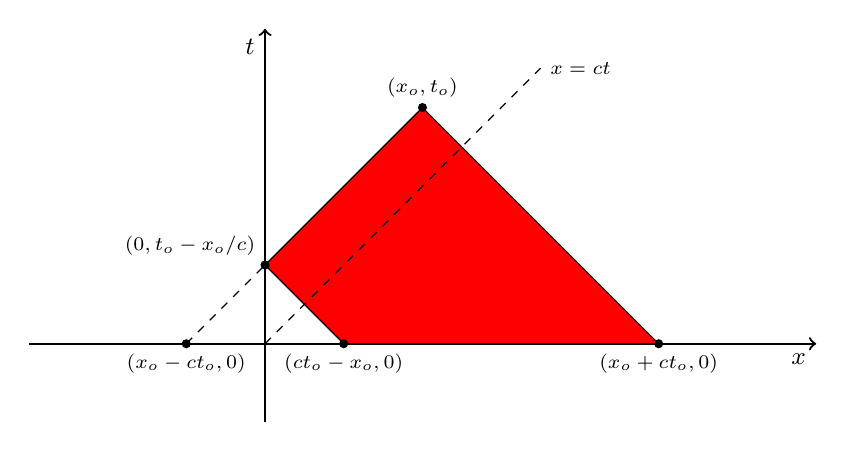
\begin{tikzpicture}
    %	\draw[help lines] (-3.5,0) grid (7,5);
    \path [fill=red] (2,3) -- (0,1) -- (1,0) -- (5,0) -- (2,3);
    \draw [->, thick] (-3,0) -- (7,0) node [below left] {\small$x$};
    \draw [->, thick] (0,-1) -- (0,4)  node [below left] {\small$t$};
    \draw [dashed] (-1,0) -- (0,1);
    \draw (0,1) -- (2,3);
    \draw (2,3) -- (5,0);
    \draw [dashed] (0,0) -- (3.5,3.5) node [right] {\scriptsize$x=ct$};
    \draw (0,1) -- (1,0);
    \draw [fill] (2,3) circle [radius=.05] node [above] {\scriptsize$(x_{o},t_{o})$};
    \draw [fill] (5,0) circle [radius=.05] node [below] {\scriptsize$(x_{o}+ct_{o},0)$};
    \draw [fill] (-1,0) circle [radius=.05] node [below] {\scriptsize$(x_{o}-ct_{o},0)$};
    \draw [fill] (0,1) circle [radius=.05] node [above left] {\scriptsize$(0, t_{o}-x_{o}/c)$};
    \draw [fill] (1,0) circle [radius=.05] node [below] {\scriptsize$(ct_{o}-x_{o},0)$};
\end{tikzpicture}

\begin{tikzpicture}
    %		%Grid
    %		\def\length{4}
    %		\draw[thin, dotted] (-\length,-\length) grid (\length,\length);
    %		\foreach \i in {1,...,\length}
    %		{
    %			\node at (\i,-2ex) {\i};
    %			\node at (-\i,-2ex) {-\i};	
    %		}
    %		\foreach \i in {1,...,\length}
    %		{
    %			\node at (-2ex,\i) {\i};	
    %			\node at (-2ex,-\i) {-\i};	
    %		}
    %		\node at (-2ex,-2ex) {0};

    %Coordinates
    \coordinate (A) at (0,0);
    \coordinate (B) at (0,3);
    \coordinate (C) at (-3,3);

    %Axis
    \draw[-latex] (-4,0) node[shift={(-0.5,0)}] {} -- (4,0) node[shift={(-0.1,-0.3)}] {$x$} node[shift={(0.5,0)}] {} ;
    \draw[-latex] (0,-1) node[shift={(0,-0.5)}] {} -- (0,4.5) node[shift={(-0.3,-0.1)}] {$y$} node[shift={(0,0.5)}] {} ;

    %Ship
    \draw[draw=black, fill=black] (A) circle (2pt);
    \draw[draw=black, fill=black] (B) circle (2pt);
    \draw[draw=black, fill=black] (C) circle (2pt);
    %%Distance
    \draw[dashed] (C) -- (A) node[pos=0.42, shift={(0,-0.5)}] {$d_3$};
    \node[right] at ($(A)!0.6!(B)$) {$d_1$};
    \draw[dashed] (B) -- (C) node[pos=0.6, above] {$d_2$};

    %Nodes
    \node[shift={(0.3,-0.3)}] at (A) {$0$};
    \node[shift={(+0.4,0)}] at (B) {$t_1$};
    \node[shift={(-0.4,0)}] at (C) {$t_2$};

\end{tikzpicture}

\begin{tikzpicture}
    \draw[-latex, thick] (-5, 0) -- (5, 0) node[shift={(-0.1, -0.3)}] {$x$};
    \draw[-latex, thick] (0, -2) -- (0, 4) node[shift={(-0.3, -0.1)}] {$y$};


\end{tikzpicture}

\begin{tikzpicture}[
        thick,
        >=stealth',
        dot/.style = {
                draw,
                fill = white,
                circle,
                inner sep = 0pt,
                minimum size = 4pt
            }
    ]
    \coordinate (O) at (0,0);
    \draw[->] (-0.3,0) -- (8,0) coordinate[label = {below:$x$}] (xmax);
    \draw[->] (0,-0.3) -- (0,5) coordinate[label = {right:$f(x)$}] (ymax);
    \path[name path=x] (0.3,0.5) -- (6.7,4.7);
    \path[name path=y] plot[smooth] coordinates {(-0.3,2) (2,1.5) (4,2.8) (6,5)};
    \scope[name intersections = {of = x and y, name = i}]
    \fill[gray!20] (i-1) -- (i-2 |- i-1) -- (i-2) -- cycle;
    \draw      (0.3,0.5) -- (6.7,4.7) node[pos=0.8, below right] {Sekante};
    \draw[red] plot[smooth] coordinates {(-0.3,2) (2,1.5) (4,2.8) (6,5)};
    \draw (i-1) node[dot, label = {above:$P$}] (i-1) {} -- node[left]
    {$f(x_0)$} (i-1 |- O) node[dot, label = {below:$x_0$}] {};
    \path (i-2) node[dot, label = {above:$Q$}] (i-2) {} -- (i-2 |- i-1)
    node[dot] (i-12) {};
    \draw           (i-12) -- (i-12 |- O) node[dot,
        label = {below:$x_0 + \varepsilon$}] {};
    \draw[blue, <->] (i-2) -- node[right] {$f(x_0 + \varepsilon) - f(x_0)$}
    (i-12);
    \draw[blue, <->] (i-1) -- node[below] {$\varepsilon$} (i-12);
    \path       (i-1 |- O) -- node[below] {$\varepsilon$} (i-2 |- O);
    \draw[gray]      (i-2) -- (i-2 -| xmax);
    \draw[gray, <->] ([xshift = -0.5cm]i-2 -| xmax) -- node[fill = white]
    {$f(x_0 + \varepsilon)$}  ([xshift = -0.5cm]xmax);
    \endscope
\end{tikzpicture}